% 3 - Technical Description. Here you explain the technical work you have carried out.
% You may include code snippets where relevant, and refer to source code in the project files.
% Try to explain the development choices you did taking into account important properties such as deployability, availability, reusability, security, modifiability, performance.

\section{Technical Description}\label{sec:technicalDescription}
In this section the technicalities of the project is explained.
First the spec will explained and then every aspect into more detail.
A flowchart of the stack can be seen below:\\
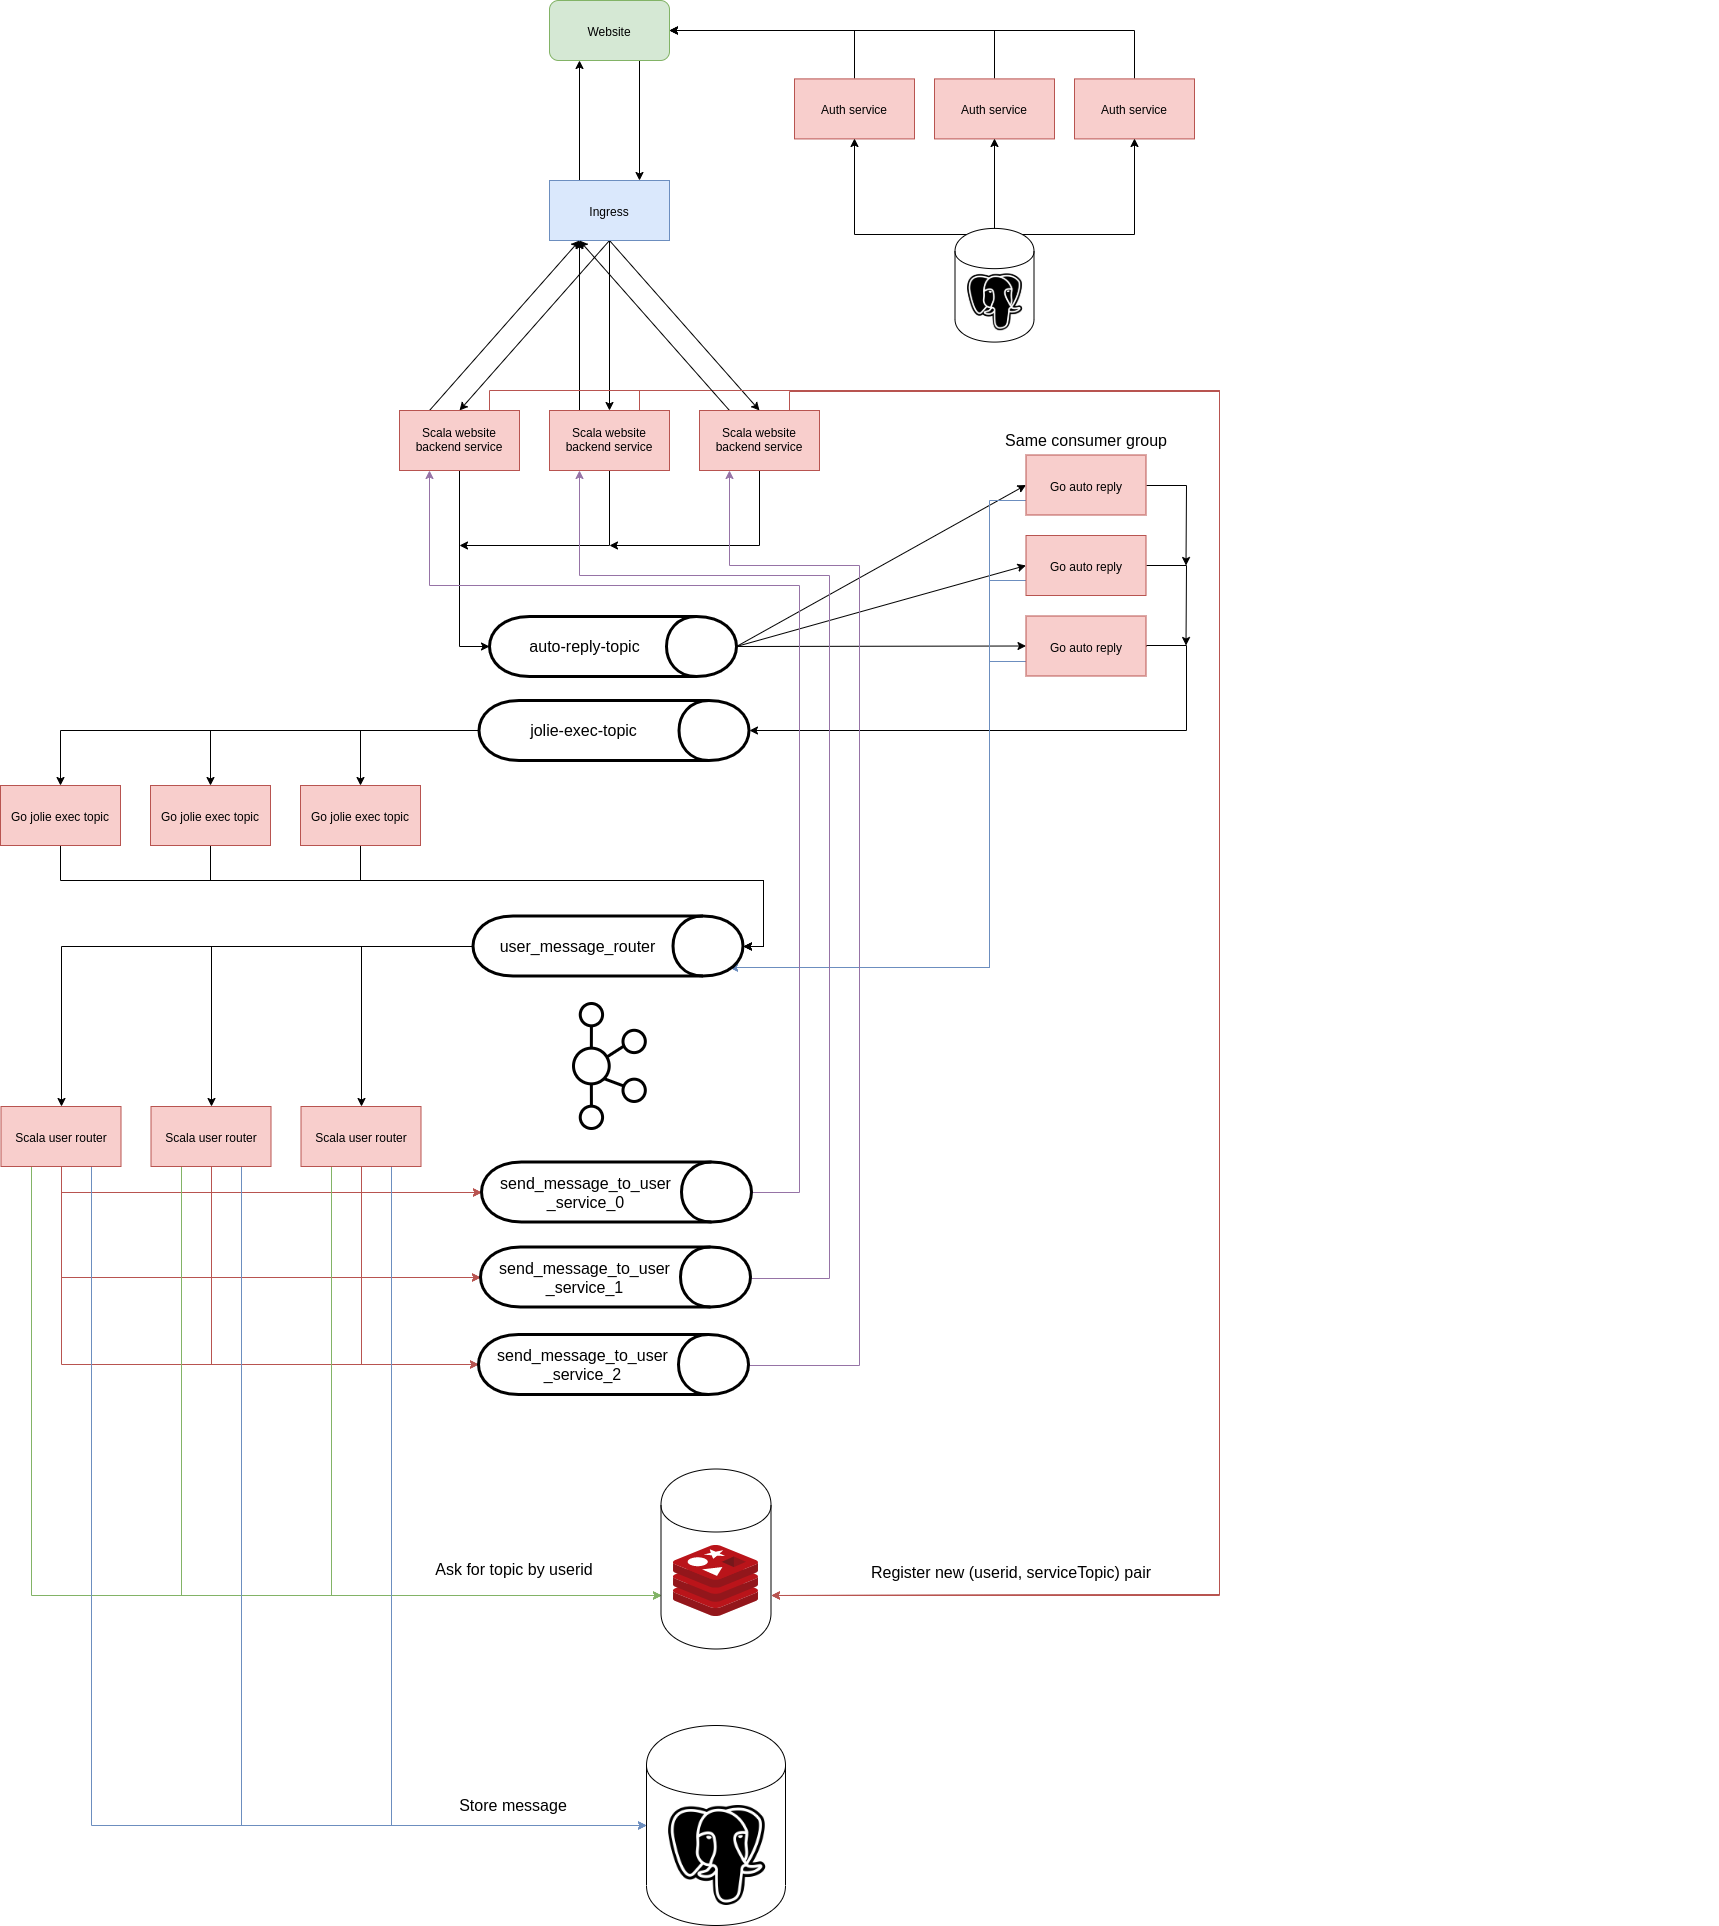
\includegraphics[scale=0.38]{stack.png}
\\
In the spec we use an event sourcing like technique.\cite{fowlerEventSourcing}
This includes a stateful data-structure that every service knows the structure of.
This structure contains any data about a message that a service would need to know, as well as the sender user.\\
\begin{lstlisting}
    {
        "messageUid": "c0a630d2-8db3-4a03-9e19-7141582f37aa",
        "sessionUid": "cf2bd7ca-ba13-40d9-8fb7-bab2064028d4",
        "messageBody": "Hello, world!",
        "senderId": 42,
        "recipientIds": [12, 8],
        "fromAutoReply": false,
        "eventDestinations": ["TOPIC1", "TOPIC2"]
    }
\end{lstlisting}
\begin{enumerate}
    \item \texttt{messageUid} a UUID that represents the message id.
    \item \texttt{sessionUid} a UUID to represent the user session (websocket session).
    \item \texttt{messageBody} this is the full message.
    \item \texttt{senderId} this is the user id of the sender.
    \item \texttt{recipientIds} these id's represent the recipient user id's.
    \item \texttt{fromAutoReply} this represents if the message was generated through pragmatic methods.
    \item \texttt{eventDestinations} this represents the topics (services) that the message must go through, usually a message ends in the router.
\end{enumerate}

\subsection{Microservices}
This section covers the responsibilities and design choices of the different microservices that comprise the chat application.

\subsubsection{Webserver (website backend)}
This service has 5 simple but important objectives.
\begin{enumerate}
    \item To serve the static single page React application.
    \item To handle user websockets through the kubernetes ingress \& insert itself as the manager of a user websocket.
    \item To check authentication when a user makes a request.
    \item To "bootstrap" a message, by inserting into one of these event sourcing models (see the JSON structure in above).
    \item To route messages back to the recipient user websockets.
\end{enumerate}
The service is written in scala and is independently scalable, has no state, storage or any stateful requirements.
It is fault tolerant and secure through JWT using HMAC256 symmetric private key encryption.

\subsubsection{Auto reply}
The auto reply service is an internal (to the cluster) service responsible for providing users with a simpler alternative to writing Jolie scripts to automate replying to messages. The feature works like how auto reply does in most e-mail clients; letting users write a static message that will be sent to everyone trying to message them. The message can be toggled on or off in the settings of the chat application.

The service is written in the Go programming language, which lends itself well to microservice development for a few reasons:

\begin{itemize}
	\item It is modern enough to have many built-in facilities useful for micro service development, like easy JSON encoding and decoding.
	\item It is a compiled language which means the service will require fewer hardware resources for the same performance.
	\item It is a strongly typed language which helps catch many bugs during compilation.
	\item Since it is developed by Google who themselves promote using a microservice architecture\cite{googlePromoteMicroservices}, there exists many tools and resources for containerizing go applications and deploying them with Kubernetes which also happens to be by Google.
\end{itemize}

State related to the auto reply service is kept in a dedicated PostgreSQL database, seperate from the service itself; this makes the service easier to scale horizontally.\cite{xenonStateless}

\subsubsection{Jolie exec}
The \texttt{Jolie-exec} service is responsible for running user-defined \textit{Jolielang} programs on incoming / outgoing messages. 
Since we use Kafka, and to have greater control of programs, the servie is implemented in \textit{Golang}, and running on an ubuntu docker image.
The service have the following goals and limitations:
\begin{itemize}
    \item Users should be able to implement an advanced auto-reply.
    \item Users should be able to programatically decide whether to recieve or discard a message.
    \item Users should be able to programatically modify outgoing message eg. adding a signature, replacing words etc.
\end{itemize}

The auto reply part allows sending an array of different messages to different recipients. 
The snippet has access to the senders id, its own id, as well as every recipients id.
With these available, it should be possible to automatically reply to regular, as well as group messages.
In the future, some anti-spam functionality should probably be implemented in the case of group messages.

A user can also implement its own message "firewall", where based on sender or content, the program can decide to \texttt{DROP} or \texttt{FORWARD} (receive) the message.

Additionally, a user can define a Jolie program to run on outgoing messages, allowing alterations of the text body before the reciver(s) see the message.

\medskip

All user-defined programs are stored in an Google Cloud Storage bucket, providing high availability, and simple integration in Golang.

For further details of implementing the Jolie program, look at the files \texttt{README.md} and the folder \texttt{examples/} of the jolie-exec repository available on GitHub\footnote{\url{https://github.com/DM874-DevOps-2019-Group-2/DM874-jolie-exec}}.

\subsubsection{Router}
The router service is responsible for routing messages to the correct services, eg the one managing the websocket for the recipient user.
The router service simply makes a lookup in redis for the key of the self-registered managed websocket, and sends the message to the found web-servers.
% static services
\subsection{Deployability}
We have chosen to use kubernetes for this project to manage almost all of our deployability.
One of the key points of kubernetes is that if your deployment configurations are written well, it handles all deployment oriented aspects.
Kubernetes is an extension to containerization, and since containerization envisions the idea of easy deployments kubernetes really pushes it to the next level.

All runtime aspects and configuration has deployability and scalability in mind, using many built-in parts of kubernetes.
We have the flexibility to say here is a service and it's configuration (which is dynamically injected at runtime if changed), now run it.
\subsection{Reusability}
Reusability is employed on two different levels.
One is the level that we re-use Kafka for every aspect of cross-service communication, meaning that kafka is the only pre-requisite to understand the communication model.

On the other side, we have services with clear API definitions.
These services can be chained in any order chosen, thus they are completely reusable if the message flow needs it.
\subsection{Performance}
Performance was a big part of our considerations, both in designing the system and the physical performance.
One of the most important parts of performance is the ability to do scaling seamlessly.
An instance of this is how we introduced a router service and a redis instance to remove the need to check all websocket managers if they managed a connection to whatever user was receiving a message.

All services are completely stateless and scalable except the websocket manager (webserver) instance, since it needs to do some rebalancing if a downscale must happen.
All services are also written in high performance asynchronous languages, which include Go and Scala.

The idea of introducing kafka has also been for performance aspects, since kafka has an obscene throughput (at least 100k req/sec without message bulking).
\subsection{Fault tolerance}
Since we have chosen to use Kafka for this project, we basically get fault tolerance for free.
Kafka is fully distributed and might be one of the most fault tolerant pieces of software out there.
It uses >2 instances of apache zookeeper, a distributed store (basically a filesystem structure) to manage the Kafka metadata.
Kafka has the ability to have multiple brokers (brokers just means instances) crash and still go on as if nothing has happened.
It uses leader election and built-in heartbeat methods which also the producers and consumers know of when connecting, and has automatic load balancing through broker rebalancing.

As stated earlier all services are completely stateless (again, escept the websocket manager), so it compliments Kafka to keep track of the messages, since Kafka is more of a log store than a traditional pub-sub.
\subsection{Monitoring}
For monitoring the system we have chosen to go the opensource, modern and standardized way with Prometheus, Grafana and Loki.
These three are an equivalent of the ELK stack, but seem to have much less resource requirements and be less of a pain to maintain.
We have used public Grafana dashboards for Kafka and Kubernetes monitoring:\\
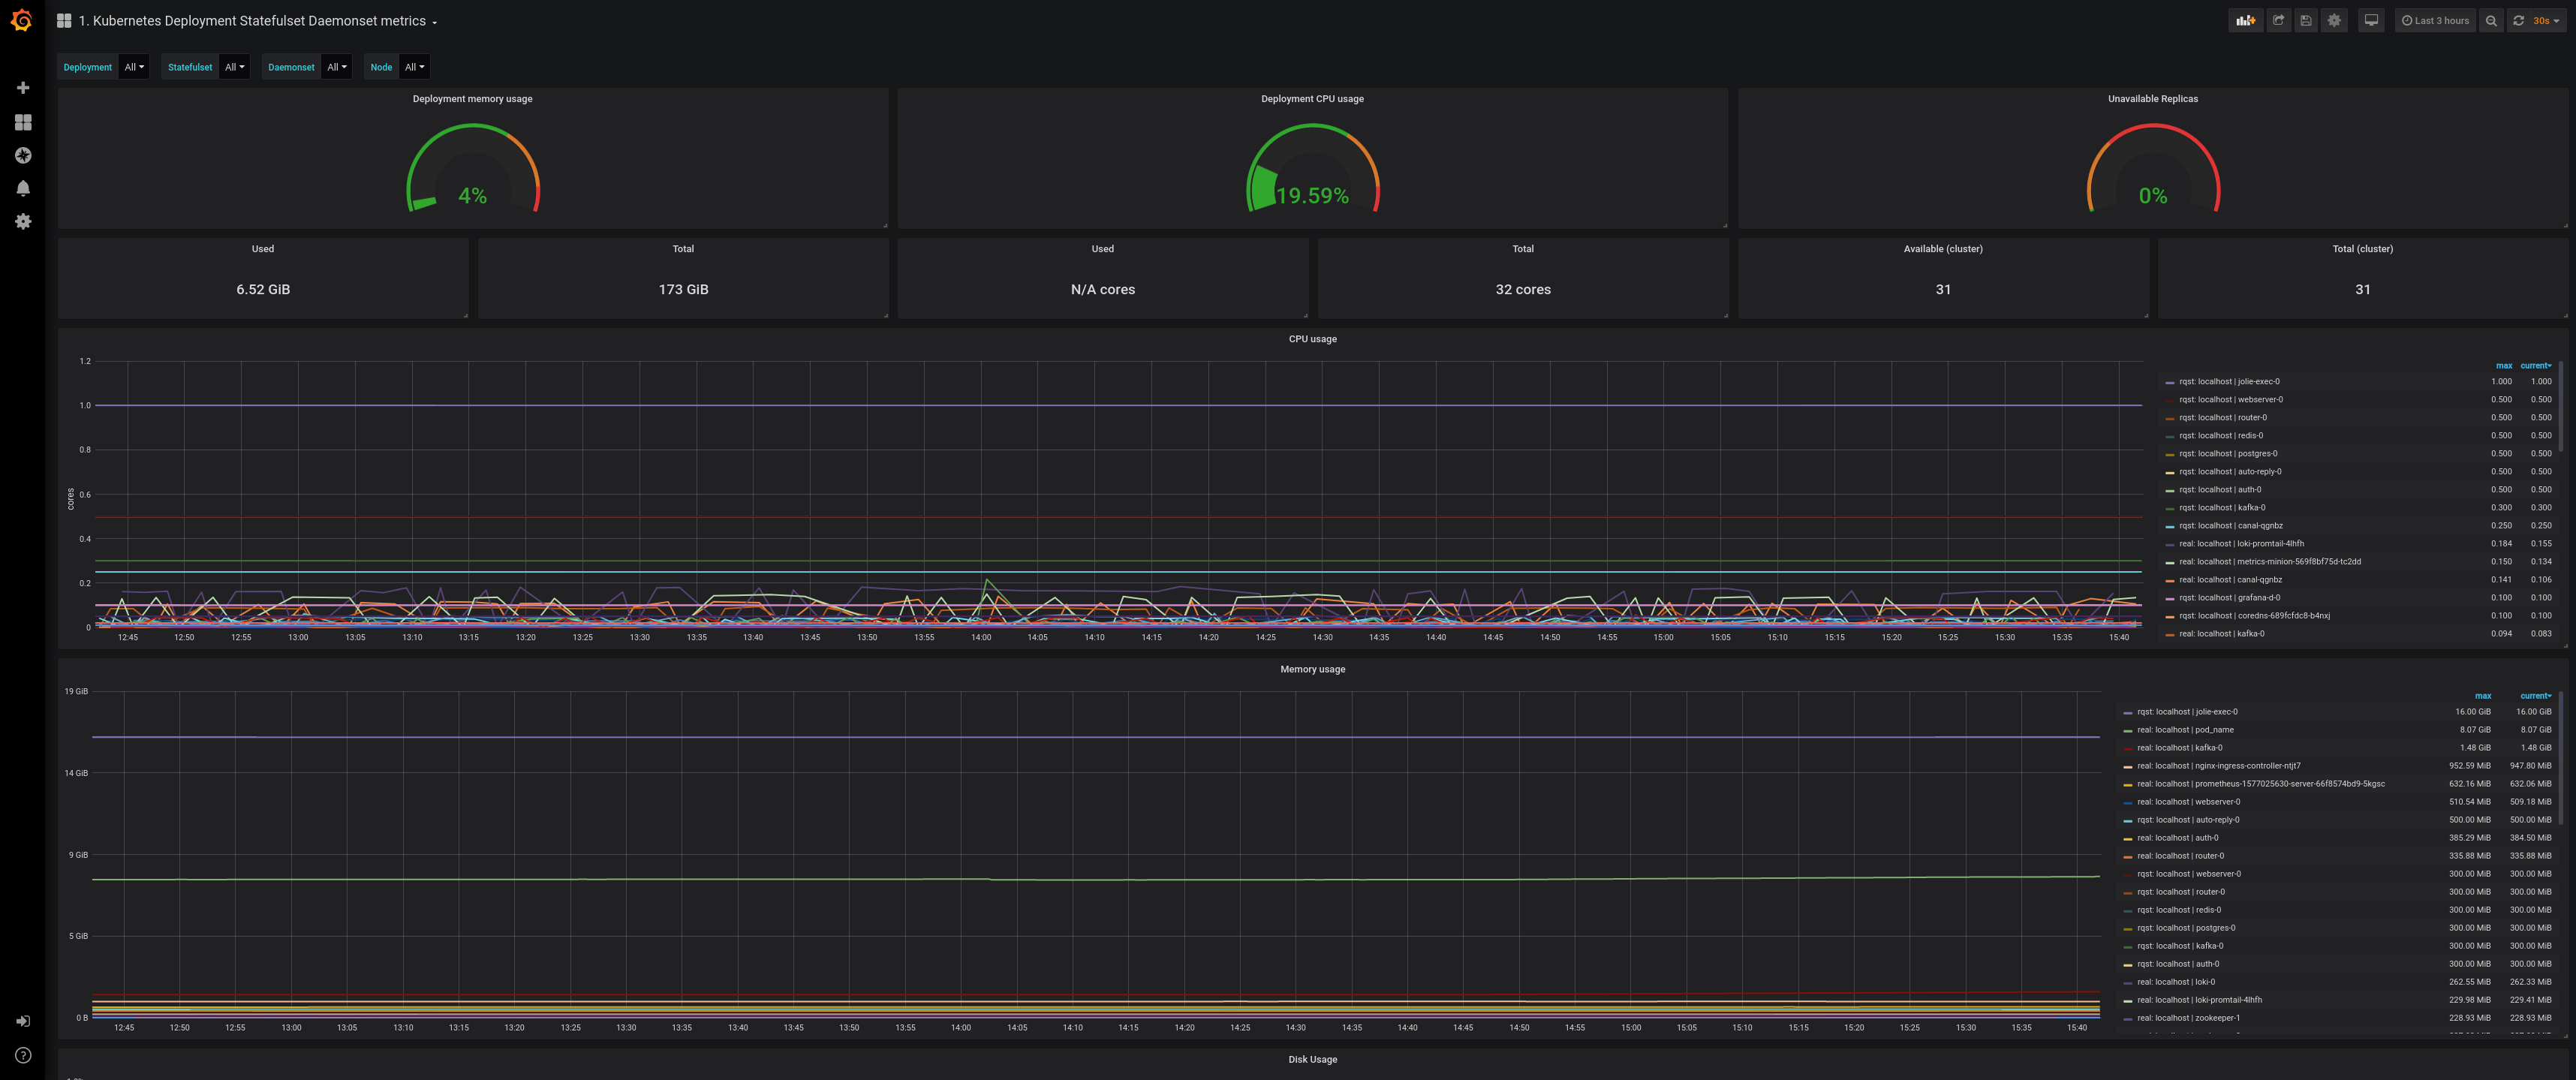
\includegraphics[scale=0.133]{grafana.png}\\
And Loki is purely log aggregation:\\
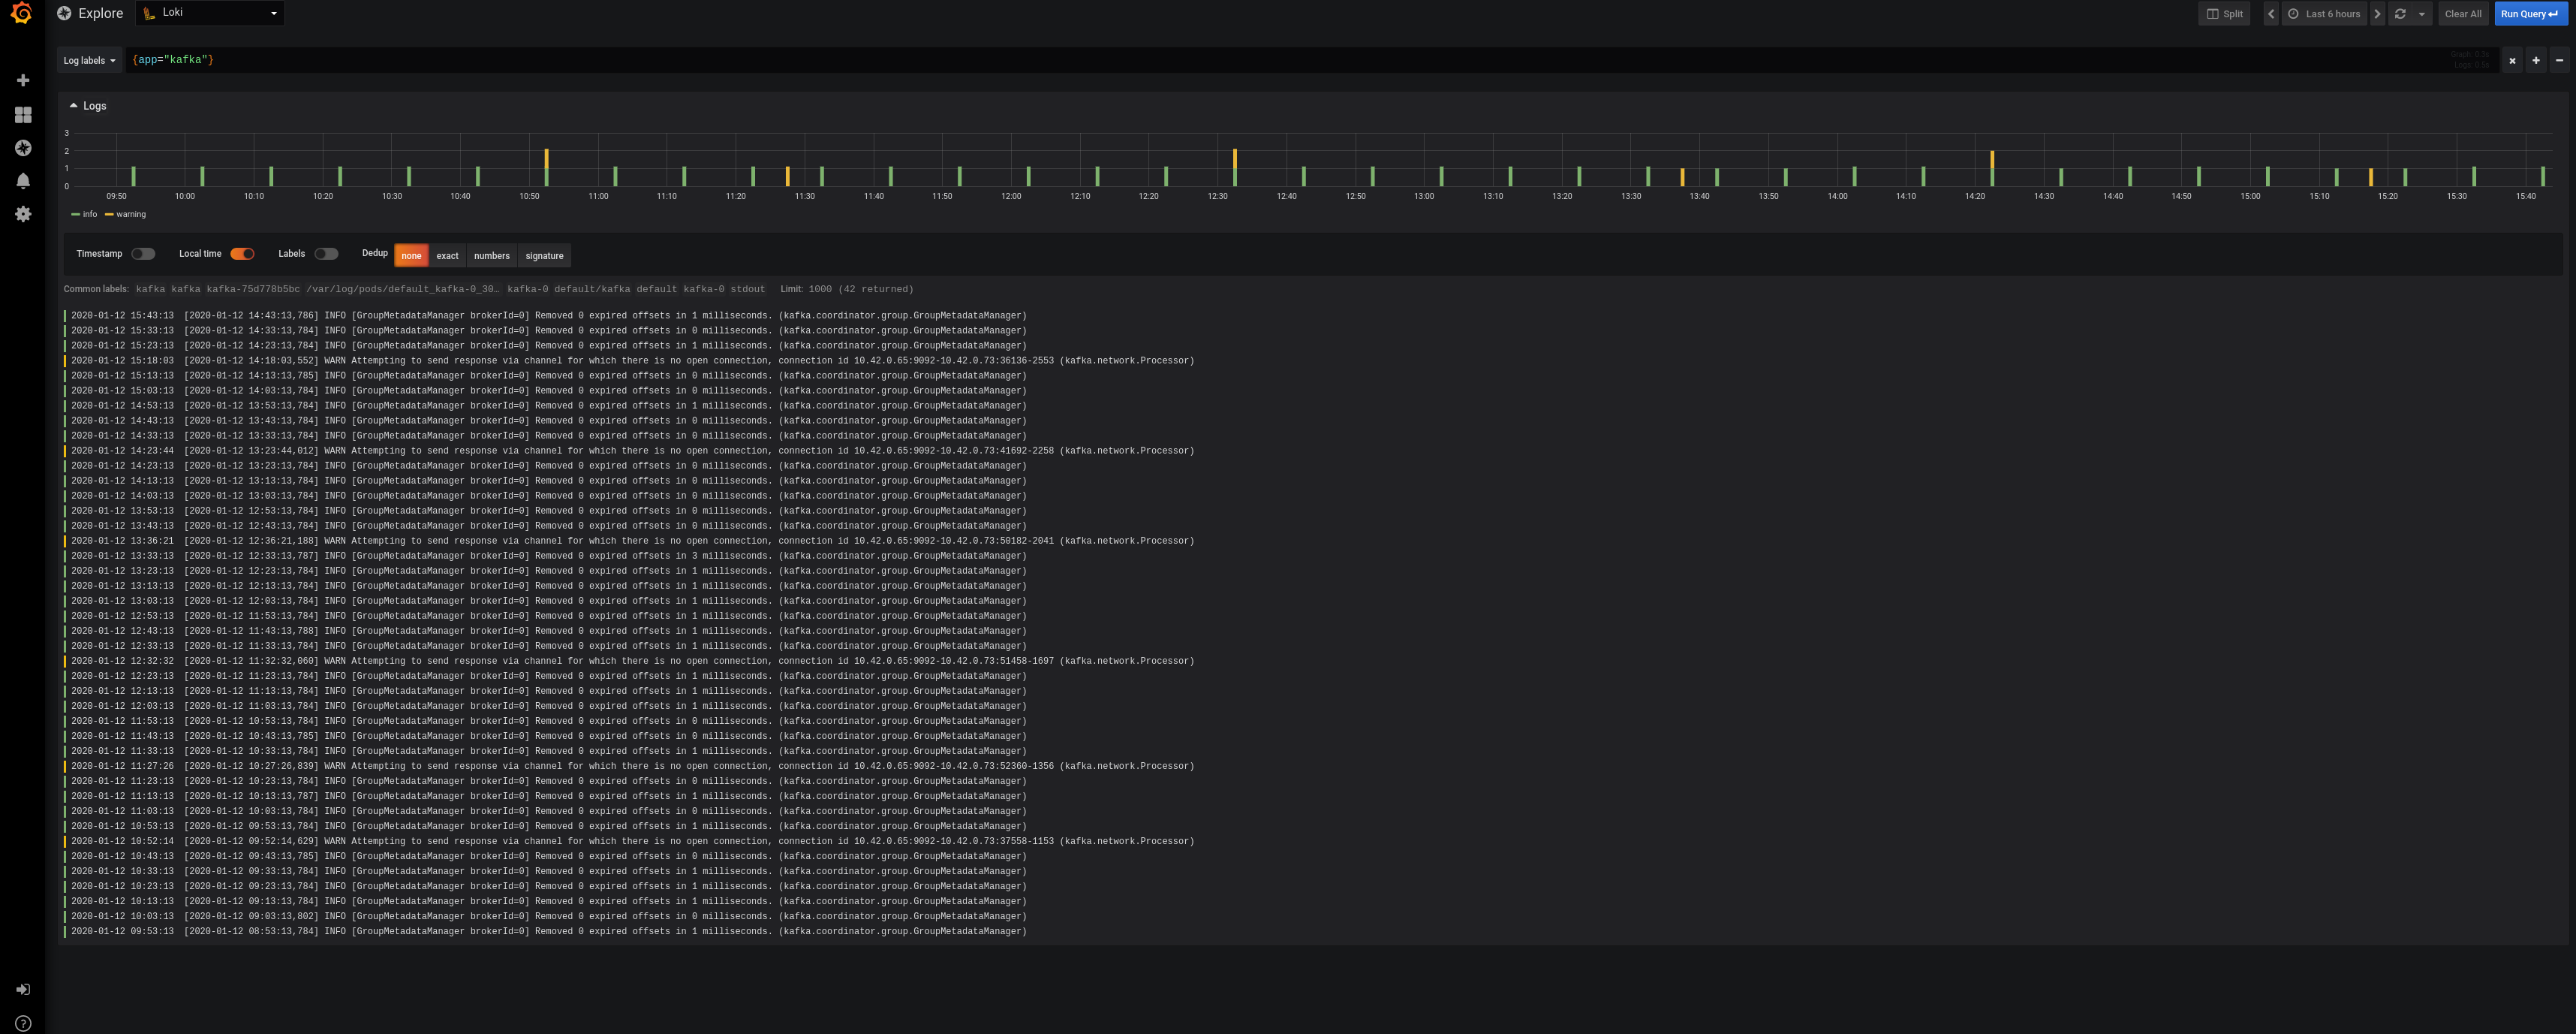
\includegraphics[scale=0.133]{loki.png}\\
